\documentclass{standalone}
\usepackage{tkz-fct}
\usepackage{tkz-euclide}
\usepackage{color}
\renewcommand*\familydefault{\sfdefault}
\usepackage{sansmath}
\usepackage{amsmath}
\sansmath
\definecolor{gray75}{gray}{0.75}
\begin{document}
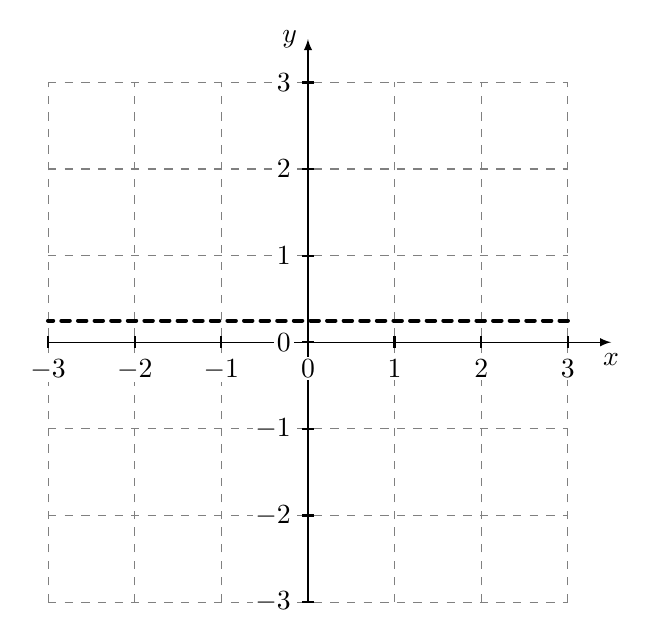
\begin{tikzpicture}[scale=1.1]
  \tkzInit[xmin=-3, xmax=3,ymin=-3,ymax=3]
  \begin{scope}[dashed]
    \tkzGrid
  \end{scope}
  \tkzDrawX[label={$x$}]
  \tkzDrawY[label={$y$}]
  \tkzLabelX
  \tkzLabelY
  \tkzFct[line width=2pt,domain=-3:3]{(x**2+1)/(4*x**2+1)}

  \tkzDefPoint(3,0.25){A}
  \tkzDefPoint(-3.0,0.25){B}
  \tkzDrawSegment[style=dashed,line width = 1.5pt](A,B)

\end{tikzpicture}
\end{document}
